\documentclass{article}

% NeurIPS 2024 style
\usepackage[final]{neurips_2024}

% Core packages
\usepackage[utf8]{inputenc}
\usepackage[T1]{fontenc}
\usepackage{graphicx}
\graphicspath{{../outputs/figures/}}
\usepackage{booktabs}
\usepackage{amsmath}
\usepackage{amssymb}
\usepackage{url}
\usepackage{hyperref}
\usepackage{microtype}
\usepackage{xcolor}
\usepackage{caption}
\usepackage{subcaption}
\usepackage{float}

\hypersetup{
  colorlinks=true,
  linkcolor=blue!60!black,
  citecolor=blue!60!black,
  urlcolor=blue!60!black
}

\title{Predicting Employee Attrition with Machine Learning:\\
Clustering, Classification, and Explainability\\
on the IBM HR Analytics Dataset}

\author{%
  \centering
  Derek Sun \quad
  Wenhai Ma \quad
  Jolin Chen \\[0.4em]
  \textit{Data Science Project, CS439} \\[0.3em]
  \small\url{https://github.com/dereksun64/IBM-HR-Attrition-Prediction}
}

\begin{document}

\maketitle

%-----------------------------------------------------------------------
\begin{abstract}
%-----------------------------------------------------------------------
Employee attrition imposes substantial financial and operational costs on
organizations, yet predicting which employees will leave remains a difficult
classification problem due to severe class imbalance and heterogeneous
workforce behavior. We present a complete machine-learning pipeline applied
to the IBM HR Analytics dataset, comprising 1,470 employees described by
35 features and exhibiting a 16.12\% attrition rate. Our pipeline spans
exploratory data analysis, SMOTE-augmented preprocessing, K-Means
unsupervised clustering for employee segmentation, and a systematic
multi-round classification study covering Logistic Regression, Random
Forest, and XGBoost under both oversampling and class-weight strategies,
followed by hyperparameter tuning, stacking, and post-hoc SHAP
explainability. K-Means clustering (k\,=\,2) reveals two latent segments
with attrition rates of 19.2\% and 9.5\%, respectively. Among all
classifiers, Logistic Regression trained with SMOTE achieves the highest
F1 score of 0.5248 with recall of 0.7872, while XGBoost after
hyperparameter tuning achieves the best ROC-AUC of 0.8132. SHAP analysis identifies OverTime, YearsWithCurrManager, and
EnvironmentSatisfaction as the top attrition drivers by feature
importance magnitude, providing actionable signals for targeted
HR intervention.
\end{abstract}

%-----------------------------------------------------------------------
\section{Introduction}
%-----------------------------------------------------------------------

Employee turnover is among the costliest challenges facing modern
organizations. Research consistently places the cost of replacing a single
employee at 50--200\% of their annual salary when recruiting costs
and lost productivity are factored in~\citep{fallucchi2020predicting,
alduayj2018predicting}. Beyond direct cost, attrition erodes institutional
knowledge and disrupts team dynamics. The ability to anticipate voluntary
departures before they occur would allow HR departments to intervene with
targeted retention programs, provided the predictive model is both accurate and interpretable.

The IBM HR Analytics dataset~\citep{ibmhr2015} provides a canonical
benchmark for this problem: 1,470 employee records, 35 features spanning
demographics, compensation, satisfaction ratings, and tenure, and a binary
attrition outcome. With only 16.12\% of employees having left (237 of
1,470), the dataset exemplifies the class imbalance that renders naive
classification approaches useless in practice. A majority-class predictor achieves 84\% accuracy while identifying zero leavers.

This paper makes three contributions:
\begin{enumerate}
  \item \textbf{Unsupervised segmentation.} K-Means clustering partitions
        employees into two latent groups with markedly different attrition
        rates (19.2\% vs.\ 9.5\%), revealing structure not visible from
        aggregate statistics alone.
  \item \textbf{Systematic classification benchmark.} We evaluate nine
        model configurations (spanning two imbalance-correction
        strategies, hyperparameter tuning, and a stacking ensemble), all
        benchmarked against a naive majority-class baseline, yielding
        clear guidance on which models and strategies best recover
        minority-class signal.
  \item \textbf{SHAP-based explainability.} Post-hoc SHAP analysis on the
        best-performing model identifies the features most responsible for
        individual predictions. The top drivers by mean $|\text{SHAP}|$ magnitude
        are OverTime, YearsWithCurrManager, and EnvironmentSatisfaction
        (directional effects verified by LR coefficients in
        Section~\ref{sec:experiments}). This enables data-driven HR
        intervention and diagnosis of systematic failure modes in the
        false-negative profile.
\end{enumerate}

The remainder of the paper is organized as follows. Section~\ref{sec:related}
reviews related work. Section~\ref{sec:data} describes the dataset and
preprocessing pipeline. Section~\ref{sec:methods} details the methodology.
Section~\ref{sec:experiments} presents experimental results, and
Section~\ref{sec:conclusion} concludes.

%-----------------------------------------------------------------------
\section{Related Work}
\label{sec:related}
%-----------------------------------------------------------------------

\paragraph{Employee and customer churn prediction.}
Machine learning has been applied extensively to churn prediction in both
HR and customer analytics contexts. \citet{alduayj2018predicting} evaluated
multiple classifiers on the IBM HR dataset and found ensemble methods
superior to single models under standard accuracy metrics. \citet{zhao2018employee}
highlighted that class imbalance is the central challenge, comparing SMOTE,
cost-sensitive learning, and decision-threshold tuning, and concluding that
no single strategy dominates across all metrics. \citet{fallucchi2020predicting}
benchmarked Logistic Regression, Decision Trees, and Random Forest on HR
data and advocated for F1 score and ROC-AUC as the only reliable indicators
when positive-class prevalence is below 20\%. Our work extends this
literature by conducting a rigorous multi-round comparison that isolates the
independent effects of imbalance-correction strategy and hyperparameter
tuning, enabling a cleaner attribution of performance differences.

\paragraph{Clustering for employee segmentation.}
Unsupervised methods have been used to identify latent employee groups
prior to supervised modeling~\citep{jain2018study}. K-Means, despite its
known sensitivity to initialization and difficulty with non-spherical
clusters, remains the dominant baseline owing to computational efficiency
and interpretability~\citep{macqueen1967}. Low silhouette scores on HR
data, a consistent finding in the literature, reflect the fact that
employee features span qualitatively different scales and do not naturally
form Euclidean clusters. We adopt K-Means for descriptive segmentation
rather than as a classification feature, using PCA projection to visualize
cluster structure and post-hoc attrition rates to interpret the groups.

\paragraph{Explainability with SHAP.}
\citet{lundberg2017unified} introduced SHAP (SHapley Additive
exPlanations), grounding feature attribution in cooperative game theory to
produce consistent, locally accurate explanations. Unlike permutation
importance, SHAP better handles correlated features than permutation importance by marginalizing
over feature interactions. This is a critical property in HR datasets where tenure,
income, and job level are heavily correlated (see Section~\ref{sec:data}).
Recent HR analytics work has demonstrated that SHAP explanations not only
improve model trust but can directly inform retention policy by identifying
high-risk feature combinations at the individual level. We apply a
LinearExplainer on our logistic regression model and examine both global
feature importance rankings and per-instance waterfall plots to diagnose
false-negative failures.

%-----------------------------------------------------------------------
\section{Dataset and Preprocessing}
\label{sec:data}
%-----------------------------------------------------------------------

\subsection{Dataset Description}

The IBM HR Analytics dataset~\citep{ibmhr2015} contains records for 1,470
employees with 35 attributes per record. Features fall into five categories:
\textit{demographic} (Age, Gender, MaritalStatus, DistanceFromHome),
\textit{job-related} (JobRole, Department, JobLevel, BusinessTravel,
OverTime), \textit{compensation} (MonthlyIncome, DailyRate, HourlyRate,
MonthlyRate, PercentSalaryHike, StockOptionLevel),
\textit{satisfaction} (JobSatisfaction, EnvironmentSatisfaction,
RelationshipSatisfaction, WorkLifeBalance, JobInvolvement), and
\textit{tenure} (YearsAtCompany, YearsInCurrentRole, TotalWorkingYears,
YearsWithCurrManager, YearsSinceLastPromotion, NumCompaniesWorked).

The binary target is \textit{Attrition} (Yes/No). As shown in
Figure~\ref{fig:imbalance}, 237 employees left (16.12\%) versus 1,233 who
stayed (83.88\%), constituting a class imbalance that makes accuracy an
unreliable performance metric.

\begin{figure}[h]
  \centering
  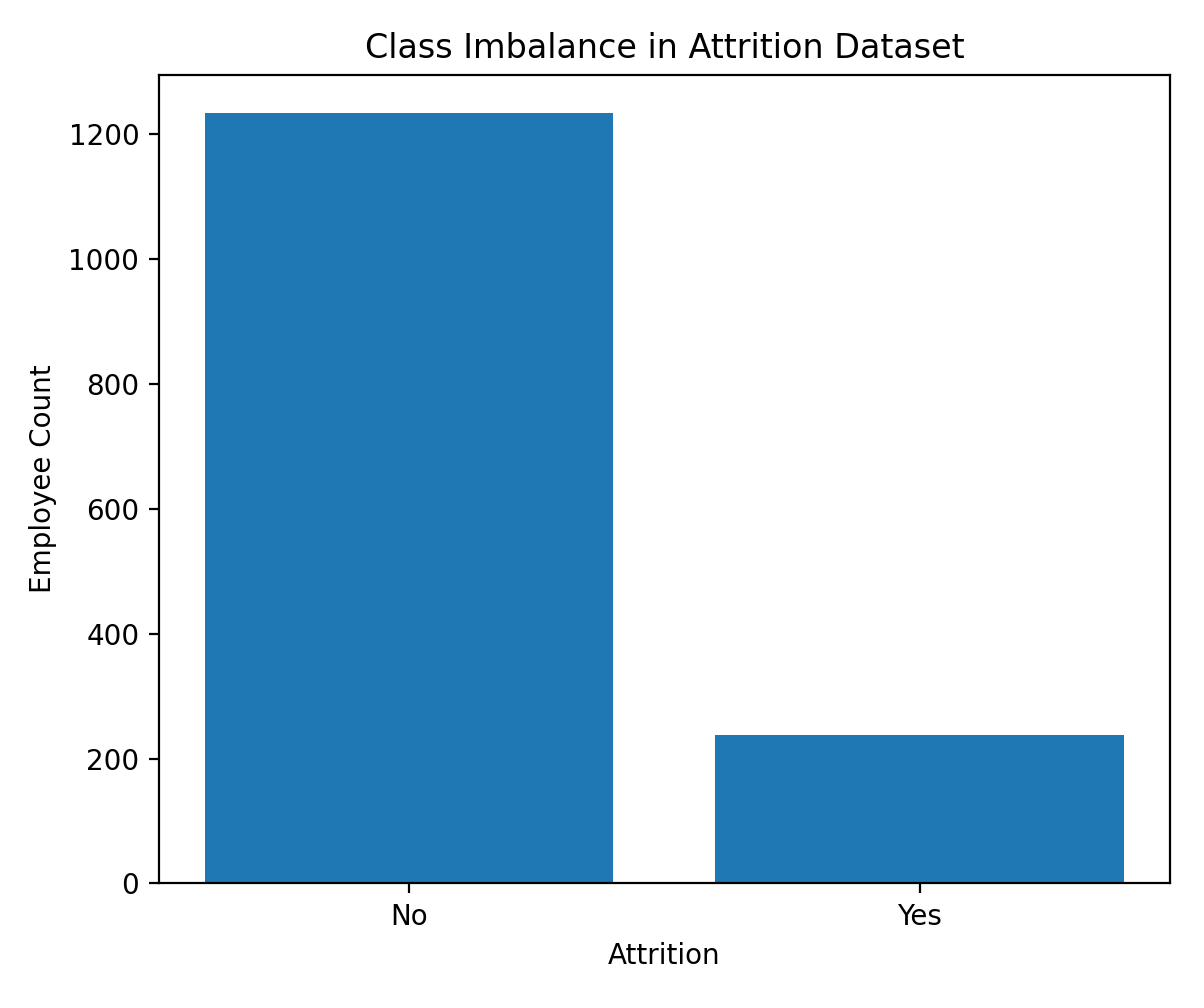
\includegraphics[width=0.55\columnwidth]{class_imbalance_plot.png}
  \caption{Class distribution of the Attrition target. Only 16.12\% of
  employees left, creating a significant imbalance that motivates
  SMOTE-based oversampling and the use of F1 and ROC-AUC as primary
  evaluation metrics.}
  \label{fig:imbalance}
\end{figure}

The dataset contains \textbf{no missing values}, as confirmed by our
automated audit (Section~\ref{sec:methods}). Four columns were dropped
during preprocessing: three constant-valued columns
(\textit{EmployeeCount}, \textit{StandardHours}, \textit{Over18}), which
carry no discriminative information, and \textit{EmployeeNumber}, a
unique employee identifier that was removed to prevent spurious
memorization of index-based patterns (identifier leakage).

\subsection{Preprocessing Pipeline}

\textbf{Encoding.} Binary categorical features (e.g., \textit{Gender},
\textit{OverTime}) were label-encoded as 0/1. Multi-class categoricals
(e.g., \textit{Department}, \textit{JobRole}, \textit{MaritalStatus},
\textit{EducationField}, \textit{BusinessTravel}) were one-hot encoded.

\textbf{Scaling.} All numeric features were standardized using
\texttt{StandardScaler} (zero mean, unit variance) after encoding.
Scaling is a strict requirement for K-Means (distance-based) and
Logistic Regression (gradient-based). Random Forest and XGBoost operate
via threshold comparisons and are scale-invariant. Their split decisions
and feature importance metrics are unaffected by linear rescaling, but
received the same preprocessed input for pipeline consistency.

\textbf{Train/test split.} We applied a stratified 80/20 split with
\texttt{random\_state=42}, yielding 1,176 training and 294 test examples,
preserving the 16.12\% attrition rate in both partitions. The test set
contains 247 employees who stayed and 47 who left.

\textbf{SMOTE.} Synthetic Minority Over-sampling Technique~\citep{chawla2002smote}
was applied exclusively to the training set after splitting. Applying SMOTE
before splitting would introduce synthetic samples into the test set,
allowing the model to ``memorize'' artificially generated minority examples
and inflate evaluation metrics, a form of data leakage. By oversampling
only the training fold, evaluation remains on the original, unaugmented
distribution.

\textbf{Correlation structure.} Figure~\ref{fig:heatmap} shows the feature
correlation heatmap. Seven pairs exceed the $|r| \geq 0.70$ threshold,
with the strongest being JobLevel--MonthlyIncome ($r = 0.950$),
JobLevel--TotalWorkingYears ($r = 0.782$), and
MonthlyIncome--TotalWorkingYears ($r = 0.773$). Permutation importance
distributes credit inconsistently among correlated features; SHAP
handles this better, which is why we use it here.

\begin{figure}[h]
  \centering
  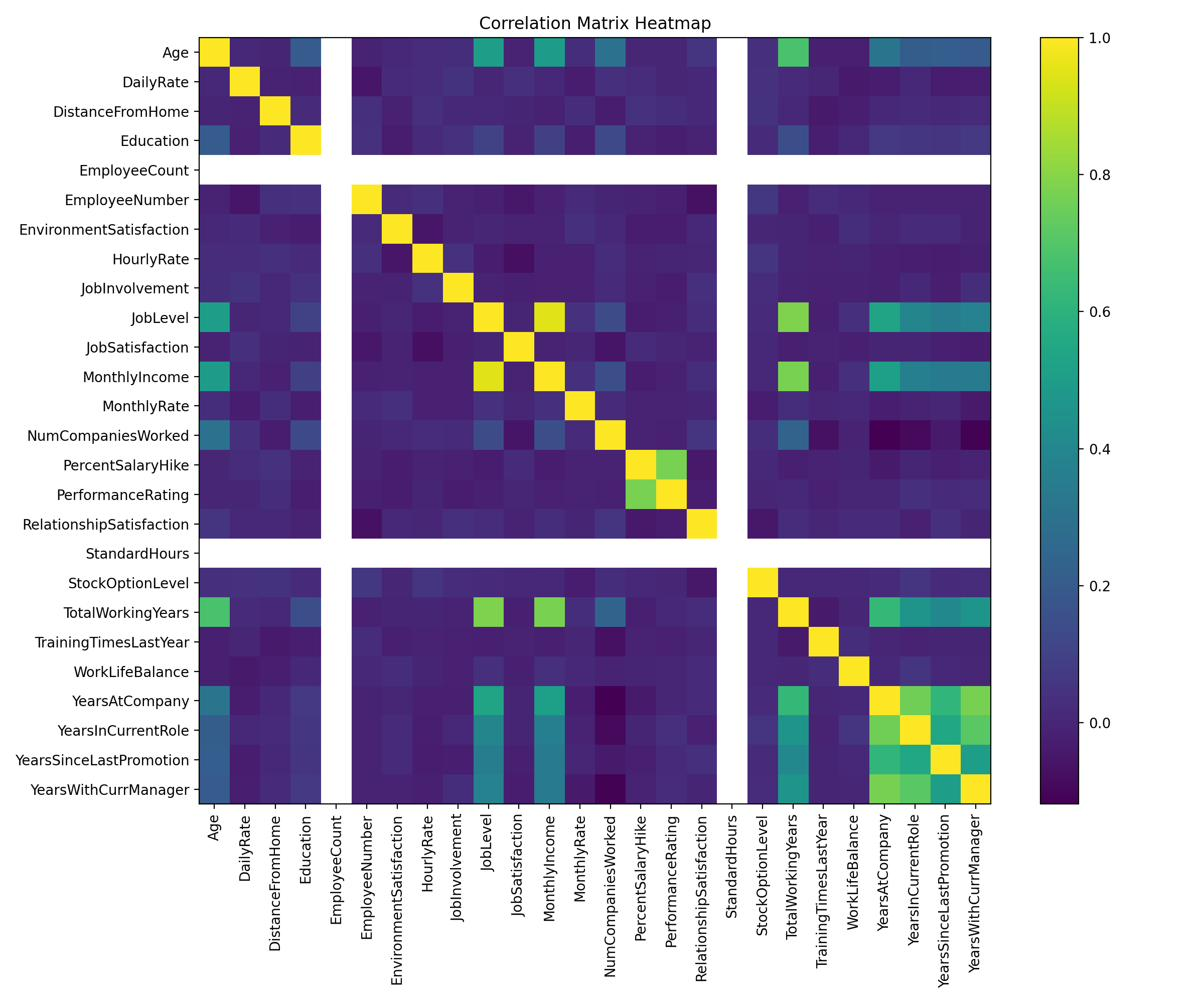
\includegraphics[width=0.85\columnwidth]{correlation_heatmap.png}
  \caption{Feature correlation heatmap. Dark red cells indicate strong
  positive correlation. Seven pairs exceed $|r|=0.70$, with
  JobLevel--MonthlyIncome showing the strongest dependence ($r=0.950$).}
  \label{fig:heatmap}
\end{figure}

%-----------------------------------------------------------------------
\section{Methodology}
\label{sec:methods}
%-----------------------------------------------------------------------

We evaluate nine model configurations across four experimental phases,
summarized in Table~\ref{tab:configs}. Each phase isolates one design
variable; all models are evaluated on the same held-out test set.

\begin{table}[h]
\centering
\caption{Overview of all nine model configurations.}
\label{tab:configs}
\small
\begin{tabular}{llll}
\toprule
\textbf{Phase} & \textbf{Models} & \textbf{Imbalance strategy} & \textbf{Cluster feature?} \\
\midrule
Round 1 & LR, RF, XGB & SMOTE (train only) & No \\
Round 2 & LR, RF, XGB & Class weights & Yes (transductive) \\
Round 3 (tuning) & RF, XGB & Class weights + RandomizedSearchCV & No \\
Round 4 (stacking) & RF + XGB$\to$LR & SMOTE (train only) & No \\
\bottomrule
\end{tabular}
\end{table}

\subsection{Naive Baseline}

Before training any learned model, we established a majority-class
baseline that always predicts \textit{Attrition = No}. On the 294-example
test set this achieves accuracy of 0.8401 while yielding F1\,=\,0.0 and
recall\,=\,0.0 (Table~\ref{tab:results}). This benchmark is essential: it
demonstrates that accuracy is a misleading metric under class imbalance and
motivates F1 score and ROC-AUC as our primary performance criteria. Any
learned model that cannot surpass this baseline on F1 has failed to recover
the minority-class signal that matters most for HR decision-making.

\subsection{Unsupervised Clustering (K-Means)}

K-Means~\citep{macqueen1967} was applied to the full scaled feature matrix
(excluding the Attrition label during fitting) to discover latent employee
segments. The number of clusters $k$ was chosen via two complementary
criteria: the \textit{elbow method}, which inspects the rate of inertia
reduction as $k$ increases, and the \textit{silhouette score}, which
measures how much better each point fits its assigned cluster than the
nearest alternative.

\begin{figure}[h]
  \centering
  \begin{subfigure}[b]{0.48\columnwidth}
    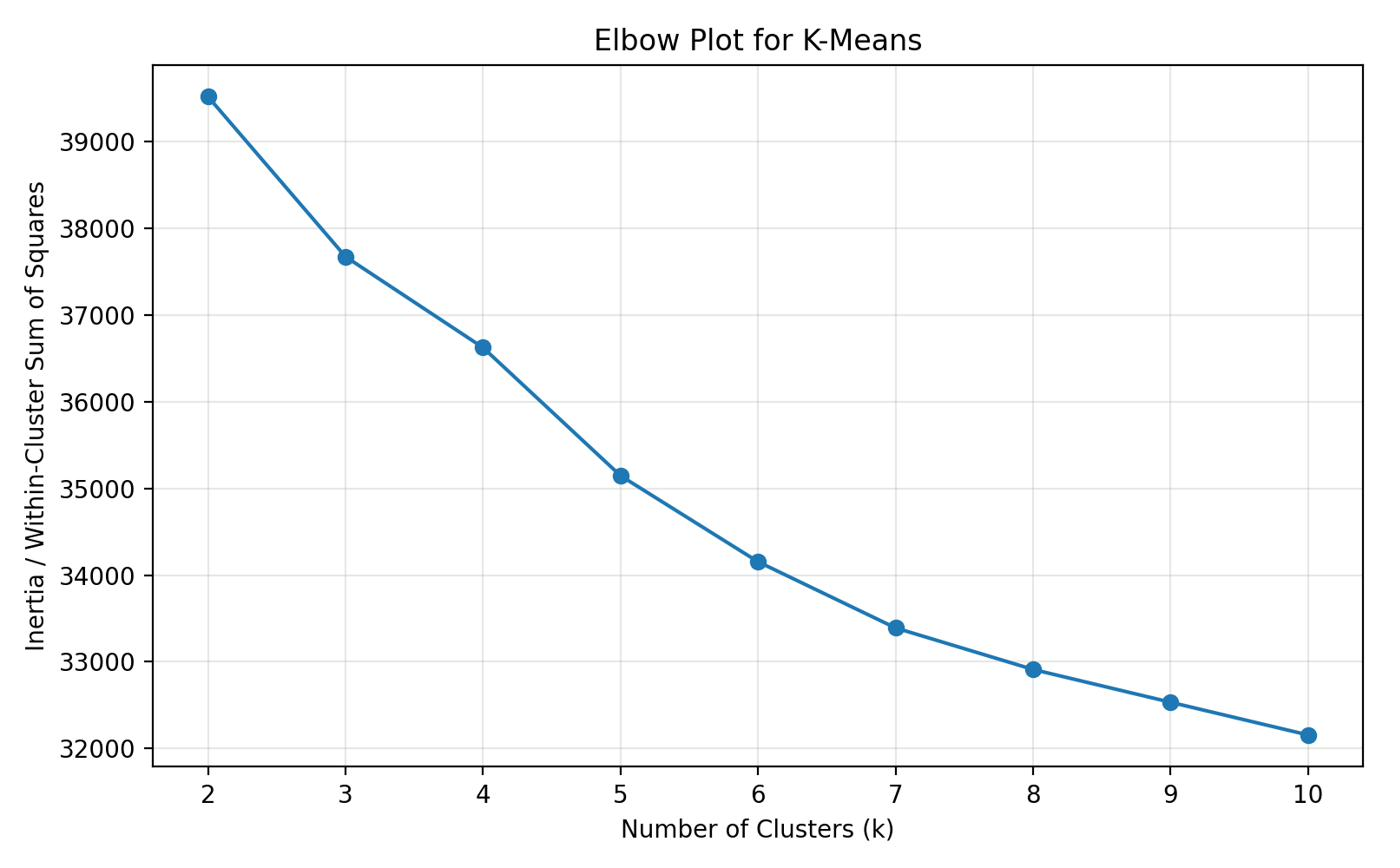
\includegraphics[width=\linewidth]{elbow_plot.png}
    \caption{Elbow plot (inertia vs.\ $k$)}
    \label{fig:elbow}
  \end{subfigure}
  \hfill
  \begin{subfigure}[b]{0.48\columnwidth}
    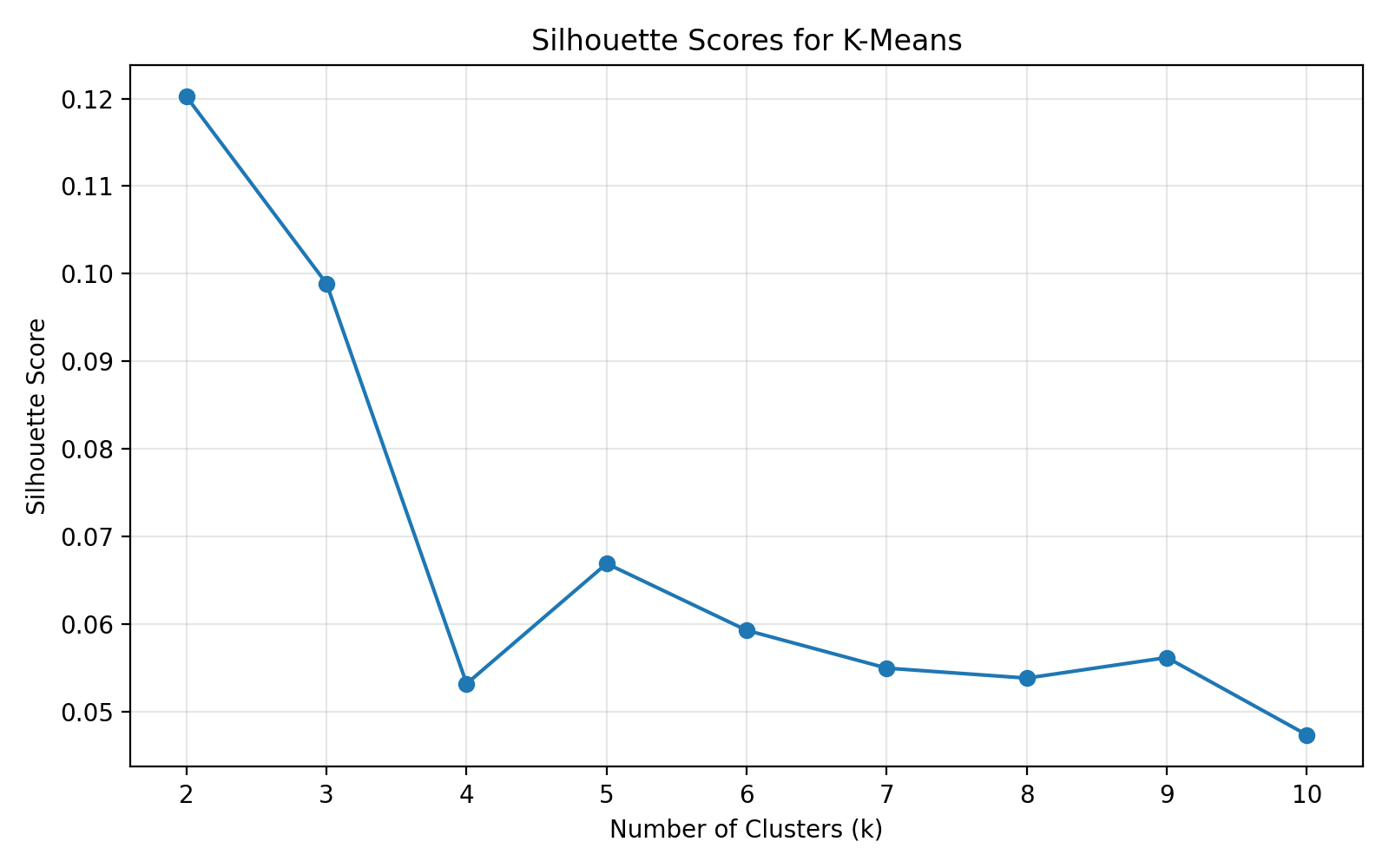
\includegraphics[width=\linewidth]{silhouette_plot.png}
    \caption{Silhouette score vs.\ $k$}
    \label{fig:silhouette}
  \end{subfigure}
  \caption{K-Means model selection over $k = 2, \ldots, 10$. Inertia at
  $k=2$ is 39{,}522; the silhouette score peaks at $k=2$ (0.1202) and
  generally declines thereafter, with minor upticks at $k=5$ (0.0669)
  and $k=9$ (0.0562), confirming $k=2$ as the overall optimal partition.}
  \label{fig:kmeans_selection}
\end{figure}

As shown in Figure~\ref{fig:kmeans_selection}, both criteria agree on
$k=2$, yielding inertia 39{,}522 and silhouette score 0.1202. In
high-dimensional HR data, employee profiles rarely form globular,
well-separated Euclidean clusters; features spanning demographics,
compensation, and tenure create a feature space where clusters are
naturally \textit{soft and overlapping}. A low silhouette score therefore
does not disqualify the result. What matters is whether the partition
provides a meaningful lift in the outcome of interest. Here it does:
Cluster~0 carries a 19.2\% attrition rate versus 9.5\% for Cluster~1,
a two-fold differential that is both substantively large and operationally
actionable even without individual-level prediction.

The cluster assignment was used \textit{only} in Round~2 (appended as an
extra feature alongside class-weight penalties) and was not included in
Rounds~1, 3 (tuning), or 4 (stacking). Clustering therefore serves
primarily as a descriptive tool for this report; the Round~2 results
incorporating the cluster label should be compared against Round~1 with
this design difference in mind.

\begin{figure}[h]
  \centering
  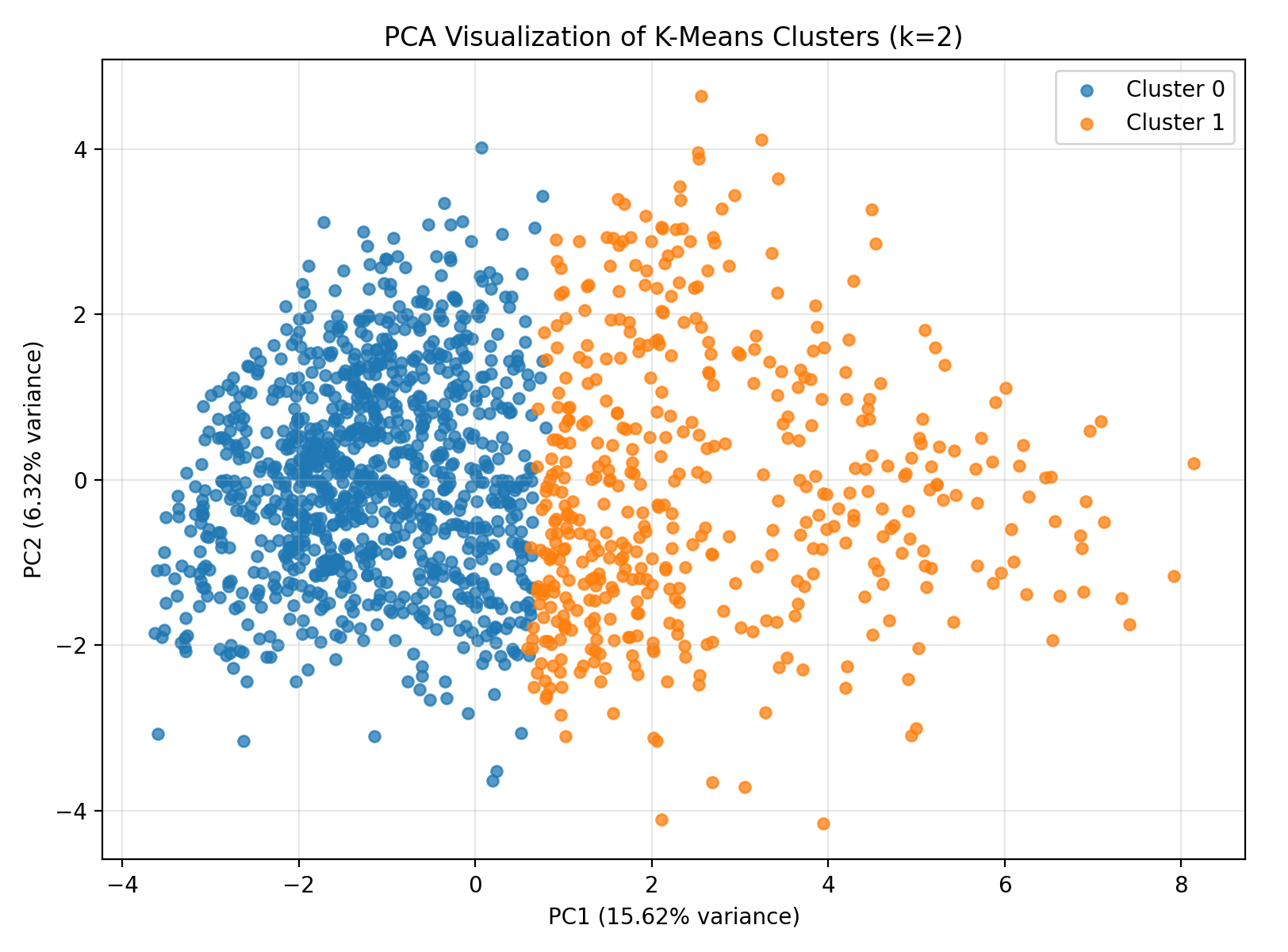
\includegraphics[width=0.72\columnwidth]{pca_cluster_plot.png}
  \caption{PCA projection of K-Means clusters ($k=2$). Cluster~0 (higher
  attrition risk, 19.2\%) and Cluster~1 (lower risk, 9.5\%) overlap
  substantially in 2D PCA space, consistent with the low silhouette score
  and the high-dimensional, mixed-scale nature of the feature set.}
  \label{fig:pca}
\end{figure}

\subsection{Classification Pipeline}

We trained three classifiers (Logistic Regression, RF, and XGBoost~\citep{chen2016xgboost}) under four successive
experimental rounds designed to isolate the effect of each design choice.

\textbf{Round 1 (SMOTE + default hyperparameters).} Models were trained on
the SMOTE-balanced training set and evaluated on the original (unaugmented)
test set. SMOTE increases minority-class representation during training
without modifying the evaluation distribution.

\textbf{Round 2 (class-weight correction + cluster feature).} The same
three models were retrained using class-weight penalties
(\texttt{class\_weight='balanced'} for LR and RF; \texttt{scale\_pos\_weight}
for XGBoost), and the K-Means cluster label was additionally appended as
a feature. Round~2 is best understood as an \textit{exploratory composite
strategy} rather than a controlled experiment: two design choices are
changed simultaneously (imbalance correction method and the addition of
a cluster feature), so individual contributions cannot be isolated from
its results alone.

The cluster label introduces a mild form of transductive leakage because
K-Means was fitted on the full 1,470-employee dataset, including test-set
employees, before the train/test split. Concretely, the cluster
assignment for a test employee was determined using that employee's own
feature values, information that would not be available to a real-time
deployment system receiving unseen data. However, in this \textit{offline
analysis} context, the cluster label serves a legitimate purpose: it acts
as a proxy for latent workforce structure, compressing the full feature
space into a single interpretable segment indicator. Round~2 metrics should
therefore be read as an upper bound on what a properly deployed cluster
feature could achieve, not as a reproducible out-of-sample estimate.

\textbf{Round 3 (Hyperparameter tuning).} The two ensemble models, RF
and XGBoost, underwent \texttt{RandomizedSearchCV} with 5-fold
cross-validation and 50 iterations. LR was excluded as a linear model
with limited hyperparameter surface. Tuned models are evaluated on the
held-out test set and compared against their Round~1 baselines throughout
(Section~\ref{sec:experiments}) to provide a consistent reference point.

\textbf{Stacking ensemble.} A meta-learner (Logistic Regression) was
trained on the out-of-fold predictions of two base learners: Random Forest
with default hyperparameters and XGBoost with tuned hyperparameters (from
Round~3). RF was left at default settings because tuning worsened its
generalization (see above); using the tuned variant as a base learner
would have embedded a worse model into the stack. The SMOTE-balanced
training set was used throughout; the cluster feature was \textit{not}
included. Note that the meta-learner (Logistic Regression) is the same
model family as LR Round~1, which is worth bearing in mind when
interpreting any advantage the stack may provide over that baseline.

%-----------------------------------------------------------------------
\section{Experiments and Results}
\label{sec:experiments}
%-----------------------------------------------------------------------

\subsection{Main Results}

Table~\ref{tab:results} reports all nine model configurations alongside the
naive baseline. Bold entries mark the best value in each column across
learned models.

\begin{table}[h]
\centering
\caption{Full results across all model configurations. Best values per
column (excluding naive baseline) are \textbf{bolded}. Primary metrics are
F1 and ROC-AUC, as accuracy is misleading under the 16.12\% attrition rate.}
\label{tab:results}
\small
\begin{tabular}{lccccc}
\toprule
\textbf{Model} & \textbf{Accuracy} & \textbf{Precision} & \textbf{Recall} & \textbf{F1} & \textbf{ROC-AUC} \\
\midrule
Naive Baseline         & 0.8401 & 0.0000 & 0.0000 & 0.0000 & 0.5000 \\
\midrule
LR Round 1 (SMOTE)     & 0.7721 & 0.3936 & \textbf{0.7872} & \textbf{0.5248} & 0.8062 \\
RF Round 1 (SMOTE)     & 0.8537 & 0.5909 & 0.2766 & 0.3768 & 0.7979 \\
XGB Round 1 (SMOTE)    & 0.8639 & 0.6296 & 0.3617 & 0.4595 & 0.7928 \\
\midrule
LR Round 2 (weights)   & 0.7653 & 0.3778 & 0.7234 & 0.4964 & 0.8173 \\
RF Round 2 (weights)   & 0.8435 & 0.5263 & 0.2128 & 0.3030 & 0.7806 \\
XGB Round 2 (weights)  & 0.8503 & 0.5600 & 0.2979 & 0.3889 & 0.8068 \\
\midrule
RF Tuned               & 0.8469 & 0.5455 & 0.2553 & 0.3478 & 0.7836 \\
XGB Tuned              & 0.8265 & 0.4643 & 0.5532 & 0.5049 & \textbf{0.8132} \\
\midrule
Stacking Ensemble      & 0.8333 & 0.4643 & 0.2766 & 0.3467 & 0.8030 \\
\bottomrule
\end{tabular}
\end{table}

\subsection{Classification Analysis}

\begin{figure}[h]
  \centering
  \begin{subfigure}[b]{0.48\columnwidth}
    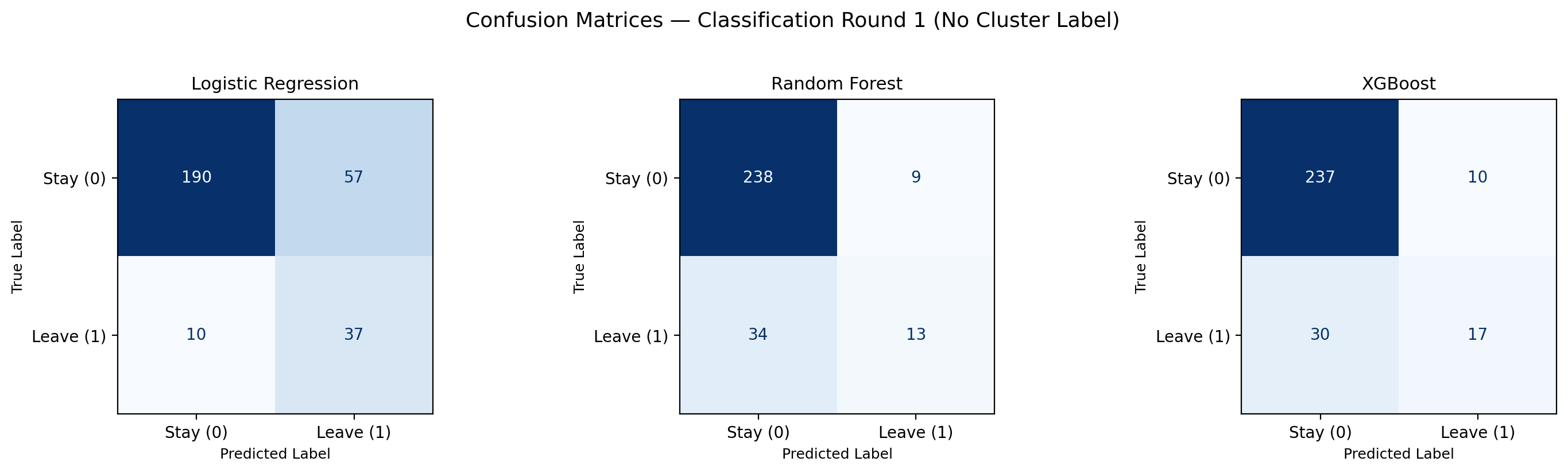
\includegraphics[width=\linewidth]{confusion_matrices_round1.png}
    \caption{Confusion matrices, Round 1}
  \end{subfigure}
  \hfill
  \begin{subfigure}[b]{0.48\columnwidth}
    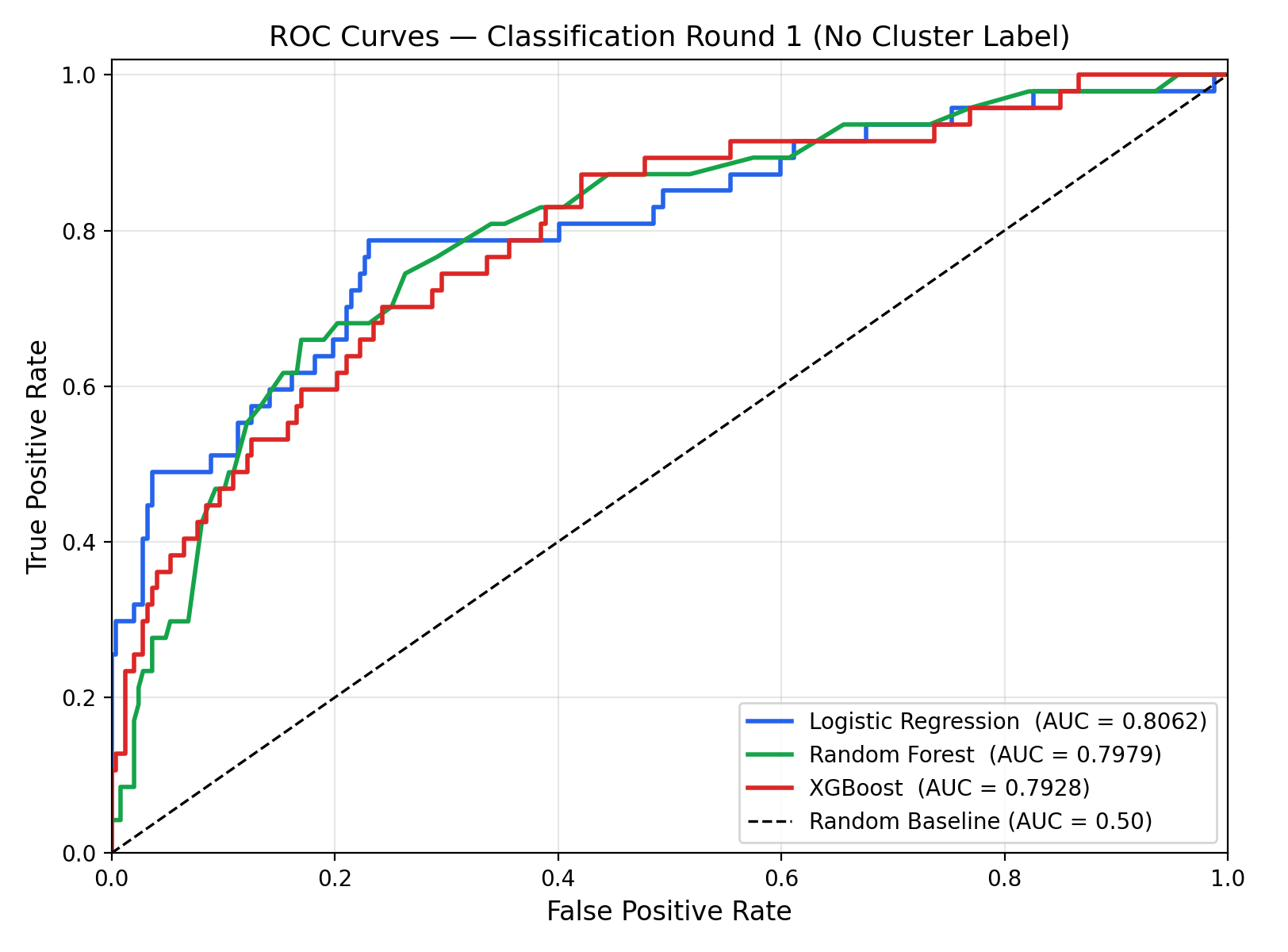
\includegraphics[width=\linewidth]{roc_curves_round1.png}
    \caption{ROC curves, Round 1}
  \end{subfigure}
  \caption{Round 1 results (SMOTE + default hyperparameters). Logistic
  Regression recovers the most true positives (37/47 leavers detected)
  at the cost of more false positives, yielding the best F1. RF and XGB
  exhibit higher precision but substantially lower recall.}
  \label{fig:round1}
\end{figure}

\textbf{Logistic Regression (Round 1) achieves the best F1 and functions
as a high-recall early-warning tool.} With F1\,=\,0.5248 and
recall\,=\,0.7872, LR Round~1 correctly identifies 37 of the 47 true
leavers in the test set (Figure~\ref{fig:round1}), a detection rate of
78.7\% compared to 0\% for the naive baseline. For HR practitioners, this
transforms an invisible problem into a manageable watchlist: the model
surfaces nearly four in five employees who will leave, enabling targeted
retention conversations before departures occur. The cost is increased false positives (57 employees incorrectly flagged), which depresses
precision (0.394) and overall accuracy (0.772). In an HR context,
however, a missed leaver is typically more costly than an unnecessary
check-in. High recall is therefore the appropriate optimization target.
SMOTE shifts the decision boundary toward the minority class by
making the positive class appear more prevalent during training, producing
the lower effective threshold that drives this recall improvement.

\textbf{XGBoost (Tuned) achieves the best ROC-AUC.} With
ROC-AUC\,=\,0.8132, XGBoost's tuned ensemble captures non-linear feature
interactions that a linear boundary cannot represent. The ROC-AUC metric
is threshold-agnostic: it measures the model's ability to rank leavers
above stayers across all thresholds. This makes XGBoost Tuned the preferred
model when downstream applications require probability scores rather than
hard predictions (e.g., for prioritizing targeted outreach).

\textbf{F1 vs.\ ROC-AUC trade-off.} These two metrics reflect different
operational priorities. When HR teams need to flag a high-coverage list
of at-risk employees (accepting some false alarms), LR Round 1 with its
recall of 0.7872 is the appropriate choice. When the goal is to rank
employees by departure probability for a constrained intervention budget,
XGBoost Tuned's ROC-AUC of 0.8132 provides the best ranking quality.

\textbf{Round 2 (exploratory composite strategy) is competitive but not
superior.} LR Round~2 achieves a ROC-AUC of 0.8173 and an F1 of 0.4964.
RF and XGB Round~2 underperform their Round~1 counterparts on F1.
As noted in Section~\ref{sec:methods}, Round~2 is an exploratory
composite: two design choices change simultaneously, making it
impossible to attribute performance differences to either factor alone.
The transductive leakage further limits generalizability, so Round~2
metrics represent an upper bound on what a properly deployed cluster
feature could achieve. The round is best read as a directional probe
suggesting that adding segment structure does not meaningfully hurt
performance, and may improve ranking quality at the margin.

\textbf{Hyperparameter tuning improves XGBoost, not RF.} Using Round~1
as the consistent baseline for both models: tuned XGBoost improves F1
from 0.4595 to 0.5049 ($+$0.045) and recall from 0.362 to 0.553,
reflecting meaningful gains from expanded search over learning rate and
tree depth. Tuned RF decreases F1 from 0.3768 to 0.3478 ($-$0.029),
suggesting Random Forest reached a local optimum under default settings
on this dataset and that further tuning did not help generalization.

\textbf{Stacking does not outperform the best single model.} The stacking
ensemble (F1\,=\,0.347, ROC-AUC\,=\,0.803) performs below both LR
Round~1 and XGBoost Tuned. Because the two base learners (RF and tuned
XGBoost) are both tree ensembles, they likely capture similar signals;
the meta-learner Logistic Regression then has little diversity to exploit.
Additionally, because LR (the meta-learner) is also the top-performing
single model, any advantage of the stack over LR Round~1 would have to
come from the base learners providing signal that LR cannot recover
alone, which does not appear to be the case here.

\begin{figure}[h]
  \centering
  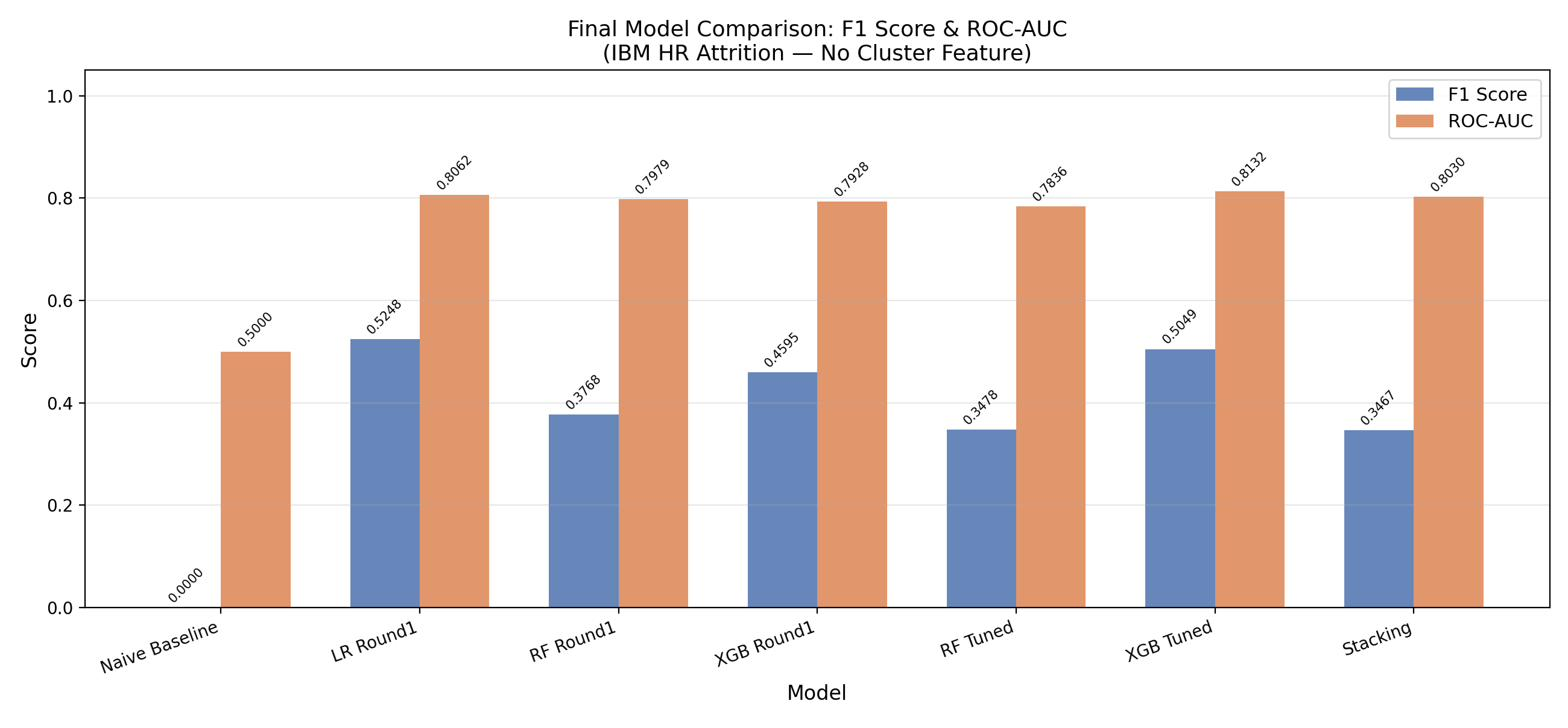
\includegraphics[width=0.82\columnwidth]{final_comparison.png}
  \caption{Comparison of model configurations on F1 and ROC-AUC, drawn
  from \texttt{final\_results\_summary.csv}. Round~2 models are excluded
  from this figure because they differ from other rounds along two
  confounded dimensions (imbalance strategy \textit{and} cluster feature);
  they are included in Table~\ref{tab:results} for completeness. LR
  Round~1 leads on F1; XGBoost Tuned leads on ROC-AUC.}
  \label{fig:final}
\end{figure}

\subsection{Clustering Results}

The K-Means partition reveals that Cluster~0 (68.4\% of employees) carries
a 19.2\% attrition rate, nearly twice the 9.5\% rate of Cluster~1
(31.6\%). While the low silhouette score (0.1202) indicates that the
clusters are not crisply separated in the feature space, the attrition
rate differential is substantial enough to be actionable: HR resources
directed at Cluster~0 members would intercept a disproportionate fraction
of eventual leavers even without individual-level prediction. The PCA
projection in Figure~\ref{fig:pca} confirms the overlap: the two clusters
are not linearly separable in 2D, which motivates the subsequent
supervised learning pipeline.

\subsection{Error Analysis}

\begin{figure}[h]
  \centering
  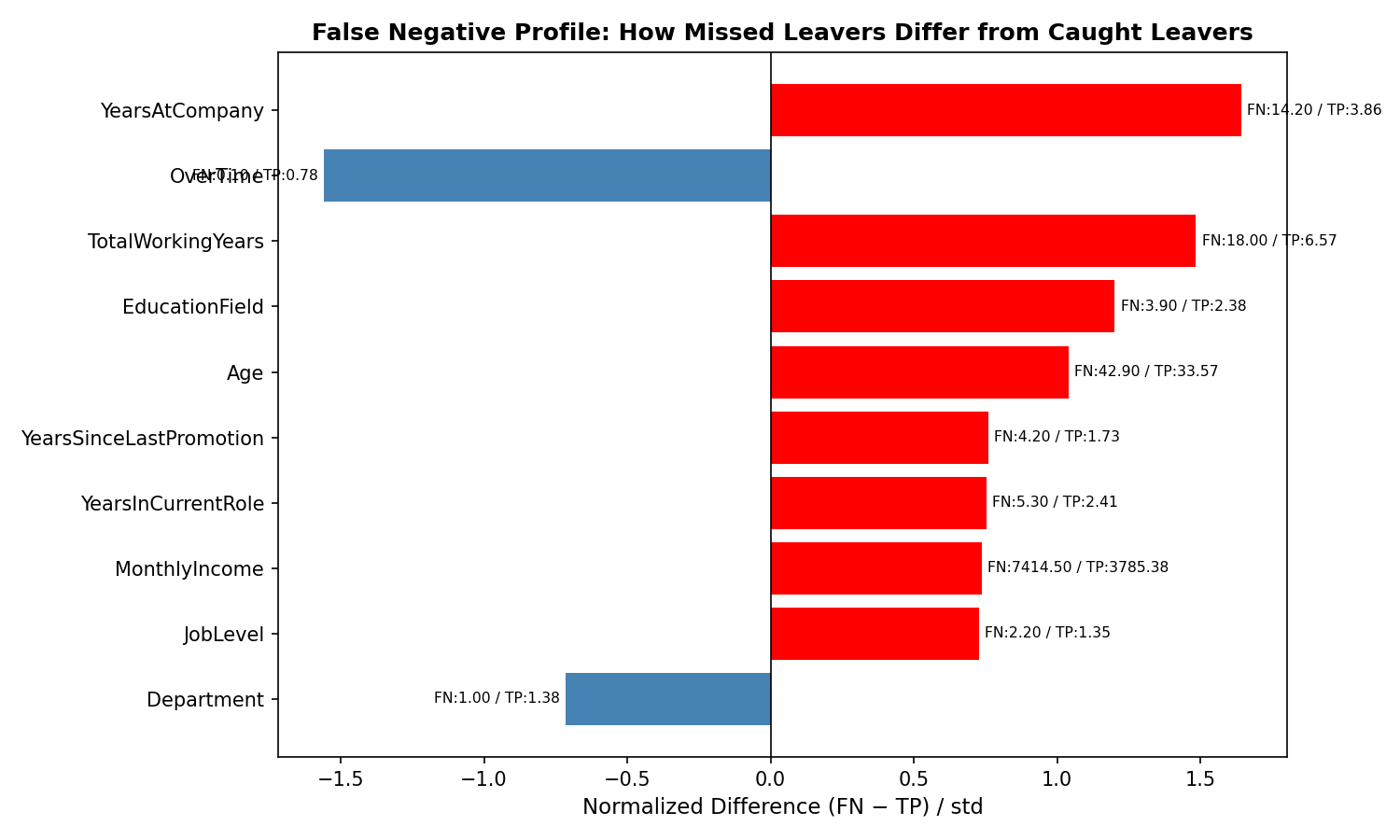
\includegraphics[width=0.72\columnwidth]{false_negative_profile.png}
  \caption{Feature profile of false negatives (employees who left but were
  predicted to stay). FN cases differ from true positives primarily along
  tenure and overtime dimensions.}
  \label{fig:fn}
\end{figure}

The LR Round~1 model produces 10 false negatives (FN) and 57 false
positives (FP) on the 294-example test set. \textbf{Model note:} the
error analysis and SHAP scripts (\texttt{error\_analysis.py},
\texttt{explainability.py}) retrain Logistic Regression with
\texttt{class\_weight=`balanced'} on top of the already SMOTE-balanced
training set, a reconstruction that differs from the Round~1 model in
Table~\ref{tab:results} (SMOTE only, no class weight). The resulting
confusion matrix is identical (37~TP, 10~FN, 57~FP, 190~TN), so
predicted labels agree, but SHAP coefficients belong to the reconstructed
variant rather than the exact Round~1 model. Figure~\ref{fig:fn} profiles
the FN subgroup against correctly identified leavers (true positives, TP).
Three features show the largest normalized divergence:
\textit{YearsAtCompany} (FN mean: 14.20 vs.\ TP mean: 3.86),
\textit{OverTime} (FN mean: 0.10 vs.\ TP mean: 0.78), and
\textit{TotalWorkingYears} (FN mean: 18.00 vs.\ TP mean: 6.57).

Categorical FN rates show concentration in certain roles: 2 of 3
Manufacturing Directors (67\%) and 1 of 1 Research Director (100\%) in
the test set were false negatives. Given the extremely small cell counts
(n\,=\,3 and n\,=\,1 respectively), these should be treated as
\textit{case studies} rather than statistically significant trends, but
they are consistent with the quantitative finding that the model
systematically underperforms on senior employees.

\textbf{Practical recommendation.} The model is highly sensitive to
burnout signals (particularly OverTime) and performs best on early-career
employees whose attrition risk is visible in structured engagement metrics.
HR teams should treat the model's output as a first-pass triage for
junior staff, while separately establishing manual monitoring programs
for high-tenure directors and senior technical leads, whose
attrition may stem from retirement planning, external poaching, or
long-term disengagement not captured by the current feature set. The
combination of model-flagged junior employees and manually monitored
senior employees would provide broader coverage than either approach
alone.

\subsection{Explainability (SHAP)}

\begin{figure}[h]
  \centering
  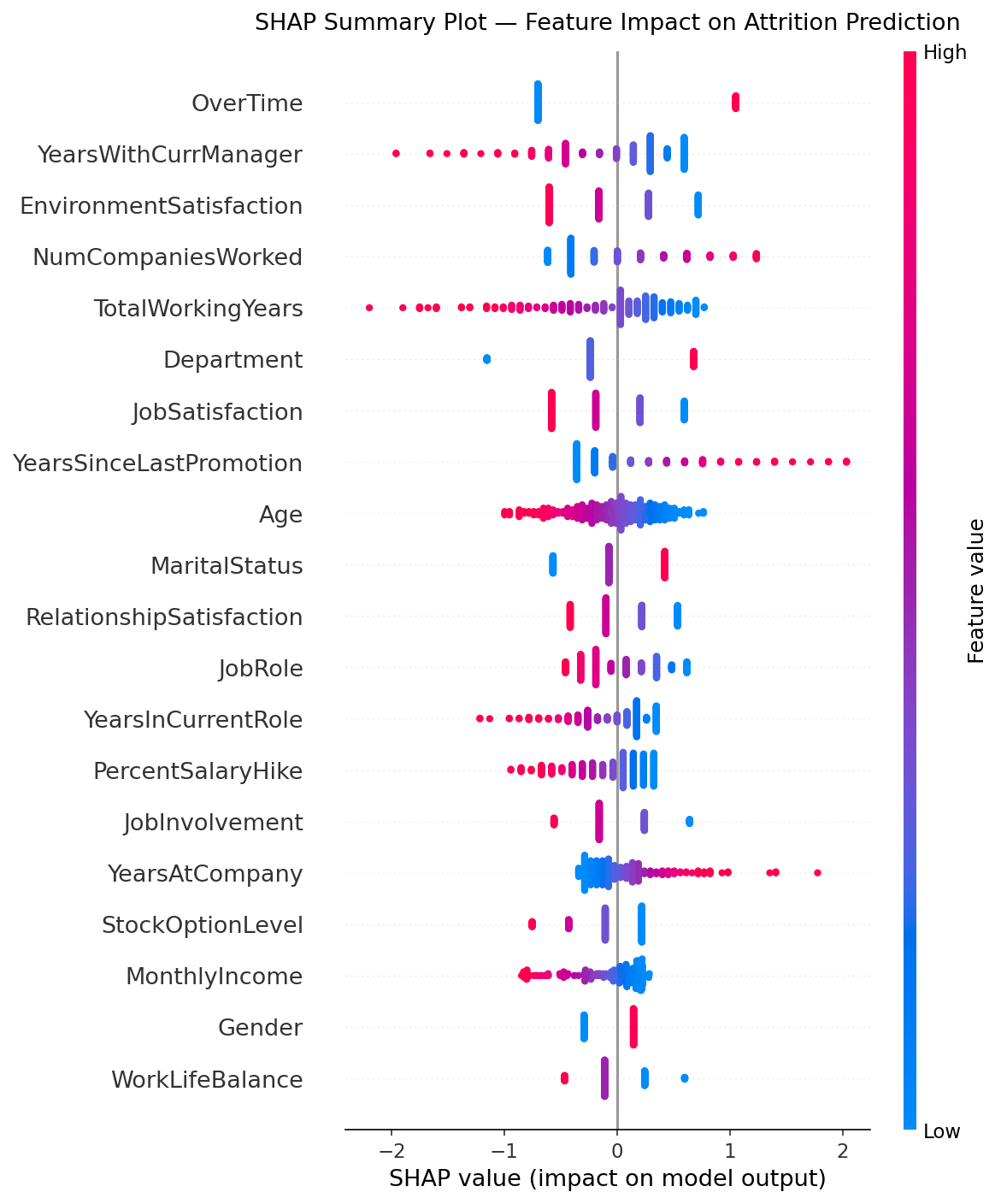
\includegraphics[width=0.95\columnwidth]{shap_summary_plot.png}
  \caption{SHAP beeswarm plot for the reconstructed LR model. Each point
  represents one test employee; color encodes feature value (red = high,
  blue = low); horizontal position encodes the SHAP contribution toward
  leaving (positive = toward leave). OverTime is the dominant driver; the
  mean $|\text{SHAP}|$ bar chart appears in Appendix~\ref{app:shap}.}
  \label{fig:shap_summary}
\end{figure}

SHAP LinearExplainer values were computed on the SMOTE-balanced training
distribution~\citep{lundberg2017unified}, using \texttt{shap\_values[1]}
throughout. Positive SHAP values indicate a push \textit{toward leaving}
(class~1); negative values indicate a push toward staying.

\textbf{Important caveat on directional inference.} Using a SMOTE-augmented
background means that for each feature, the SHAP baseline is the feature's
mean across synthetic-plus-real training samples rather than real employees
alone. SMOTE interpolates new minority-class points between existing ones,
which can shift the synthetic distribution's feature means away from the
real population mean. As a result, a feature may appear to have a positive
mean SHAP value (implying it increases attrition risk) simply because the
real test set has a \textit{lower} mean for that feature than the inflated
SMOTE baseline, rather than because the feature actually increases risk in the
model. This artifact affected YearsWithCurrManager in our analysis, where
the mean SHAP sign was positive (suggesting increased risk) despite the LR
coefficient being negative ($\beta = -0.536$, decreasing risk). Throughout
this section, \textbf{directional influence is verified by the LR
coefficients ($\beta$)}, which are unaffected by the background
distribution. Mean $|\text{SHAP}|$ values are used only to rank
\textit{magnitude} of influence.

Figure~\ref{fig:shap_summary} and Appendix~\ref{app:shap} reveal a
clear hierarchy of feature influence. \textbf{OverTime} is by far the
strongest predictor (mean$|\text{SHAP}|$\,=\,0.793): working overtime
substantially increases predicted attrition probability, consistent with
literature on work--life balance burnout. \textbf{YearsWithCurrManager}
(0.445) is the second-ranked feature by mean $|\text{SHAP}|$. Its LR
coefficient is $\beta = -0.536$, indicating that longer tenure with the
current manager \textit{decreases} predicted attrition risk, consistent
with the interpretation that an established manager relationship provides
stability. The positive mean SHAP sign reported in the summary file
reflects a SMOTE-background artifact (the synthetic training distribution
has a higher mean for this feature than the real test set), and the
coefficient is the correct directional reference. \textbf{EnvironmentSatisfaction}
(0.438) decreases attrition risk when high ($\beta = -0.480$). \textbf{NumCompaniesWorked}
(0.437) increases attrition risk when high ($\beta = +0.511$), consistent
with the job-hopper pattern: employees with a history of frequent employer
changes leave more readily. \textbf{TotalWorkingYears} (0.429) decreases
risk when high ($\beta = -0.579$), indicating that more experienced
employees exhibit lower attrition propensity on average.

Waterfall analysis of a representative false-negative case shows the
competing SHAP forces that caused a misclassification. Under the
positive-class sign convention, OverTime ($-0.702$) and Age ($-0.653$)
pushed \textit{toward staying}, while EnvironmentSatisfaction ($+0.721$)
simultaneously pushed \textit{toward leaving}. The net prediction was
``stay'' because the staying-signals collectively outweighed the leaving-signal,
masking the true attrition outcome. In contrast, a correctly identified
leaver received a strong net push toward leaving: OverTime ($+1.054$)
and TotalWorkingYears ($+0.625$) drove the prediction upward while
NumCompaniesWorked ($-0.615$) partially offset them, but the positive
signals dominated ($+1.054 + 0.625 - 0.615 = +1.064$ net), yielding a
confident correct prediction. This per-instance view underscores why
global importance rankings are insufficient: competing SHAP effects can
cancel at the instance level, and waterfall plots are the appropriate
diagnostic for borderline or missed cases.

%-----------------------------------------------------------------------
\section{Conclusion}
\label{sec:conclusion}
%-----------------------------------------------------------------------

We presented a complete machine-learning pipeline for employee attrition
prediction on the IBM HR Analytics dataset. Among nine model configurations
benchmarked against a majority-class baseline (F1\,=\,0), Logistic
Regression trained with SMOTE achieved the best minority-class recovery
(F1\,=\,0.5248, recall\,=\,0.7872), detecting 78.7\% of leavers and
serving as a practical high-recall early-warning tool for HR teams.
XGBoost after hyperparameter tuning achieved the best probability ranking
quality (ROC-AUC\,=\,0.8132), making it the preferred model for
constrained intervention budgets. K-Means clustering revealed two latent
employee segments with attrition rates of 19.2\% vs.\ 9.5\%, providing
an actionable segmentation even with a low silhouette score. SHAP
analysis (with directional effects verified by LR coefficients to avoid
SMOTE background artifacts) identified OverTime ($\beta=+0.796$, increases
risk), YearsWithCurrManager ($\beta=-0.536$, decreases risk), and
EnvironmentSatisfaction ($\beta=-0.480$, decreases risk) as the top three
drivers by mean $|\text{SHAP}|$ magnitude. Error analysis revealed
that the model systematically misses longer-tenured, low-overtime
employees, motivating a hybrid monitoring strategy that combines
model-flagged junior staff with manual oversight of senior roles. For
future deployments, sweeping the classification threshold on a held-out
validation set (rather than using the default 0.5) would be the
single highest-leverage improvement available without retraining any model.

\textbf{Limitations.} Four limitations should be acknowledged.
(1) \textit{Weak clustering cohesion:} the silhouette score of 0.1202
is low, consistent with published HR clustering studies where mixed-scale
tabular data rarely produces scores above 0.25 \citep{jain2018study}.
Density-based methods such as HDBSCAN may be better suited to this
feature space. (2) \textit{Single train/test split:} all metrics in
Table~\ref{tab:results} derive from one 80/20 split. With only 47
positive examples in the test set, a difference of one or two correct
predictions shifts F1 by $\approx 0.02$--$0.04$; repeated stratified
$k$-fold cross-validation (e.g., $5{\times}5$) would be needed to report
mean\,$\pm$\,std and confirm that differences between models are not
split-specific noise. (3) \textit{F1 ceiling at $\approx 0.52$:}
despite multiple tuning rounds, F1 did not exceed 0.53, suggesting the
available features do not fully capture latent attrition causes.
(4) \textit{SMOTE-induced boundary distortion and background mismatch:}
synthetic samples may not lie on the true data manifold, potentially
distorting the decision boundary; additionally, using the SMOTE set as
the SHAP background distribution (rather than the original training data)
may shift feature attribution baselines.
(5) \textit{Fixed classification threshold:} all precision, recall, and
F1 values are reported at the default 0.5 decision threshold. With
SMOTE-shifted decision boundaries, this threshold is rarely optimal for
imbalanced problems; a validation-set threshold sweep could meaningfully
improve F1 and recall without retraining any model.

\textbf{Future directions.} (1) \textit{Feature engineering:} interaction
terms (e.g., OverTime $\times$ JobSatisfaction) and SHAP-guided feature
selection could reduce noise and amplify discriminative signal.
(2) \textit{Alternative models:} CatBoost or a neural network
with dropout regularization may better handle the feature correlations
and non-linear interactions present in HR data. (3) \textit{Longitudinal
modeling:} a single cross-section captures only a snapshot; survival
analysis or recurrent models trained on monthly employee snapshots
would better capture the temporal dynamics of attrition risk and enable
early intervention \textit{before} disengagement becomes irreversible.
(4) \textit{Precision-recall curves and threshold tuning:} for an imbalanced
problem with a 16\% positive rate, precision-recall curves are more
informative than ROC curves because they directly show the trade-off in
the minority class. Adding PR curves for LR Round~1 and XGB Tuned, and
sweeping the classification threshold on a validation set, would
strengthen the experimental section and likely improve reported F1.

%-----------------------------------------------------------------------
\bibliographystyle{plainnat}
\bibliography{references}

%-----------------------------------------------------------------------
\appendix
\section{SHAP Feature Importance Bar Chart}
\label{app:shap}
%-----------------------------------------------------------------------

\begin{figure}[h]
  \centering
  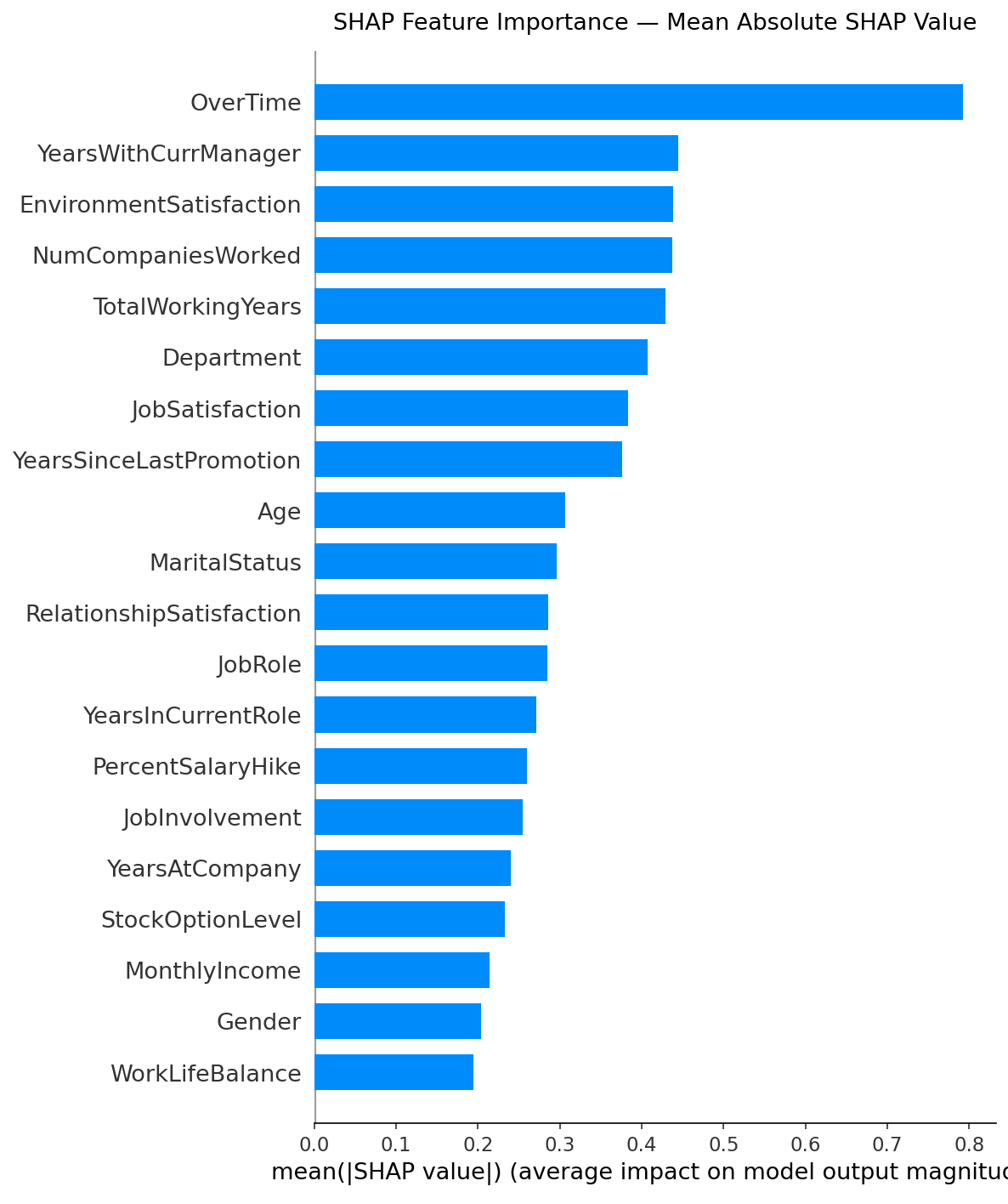
\includegraphics[width=0.72\columnwidth]{shap_feature_importance.png}
  \caption{Global SHAP feature importance (mean $|\text{SHAP}|$) for the
  reconstructed LR model. Top five features by magnitude: OverTime (0.793),
  YearsWithCurrManager (0.445), EnvironmentSatisfaction (0.438),
  NumCompaniesWorked (0.437), and TotalWorkingYears (0.429).
  \textbf{Warning:} while mean $|\text{SHAP}|$ correctly indicates
  \textit{importance magnitude}, the direction of influence should not
  be inferred from SHAP sign here. The SMOTE background distribution
  can invert the sign relative to the true model direction. Directional
  effects are verified by LR coefficients ($\beta$) as reported in
  Section~\ref{sec:experiments}.}
  \label{fig:shap_importance}
\end{figure}

\end{document}
